\documentclass[12pt]{article}

% JASA necessities --------
% NOTE: To produce blinded version, replace "1" with "0" below.
\newcommand{\blind}{1}
\pdfminorversion=4
% DON'T change margins - should be 1 inch all around.
% Daniel: This stuff seems not to have that effect despite the JASA
% template's claim (the bottom margin is huge)
% \addtolength{\oddsidemargin}{-.5in}%
% \addtolength{\evensidemargin}{-.5in}%
% \addtolength{\textwidth}{1in}%
% \addtolength{\textheight}{-.3in}%
% \addtolength{\topmargin}{-.8in}%
\usepackage[margin=1in]{geometry} % use this instead

\def\spacingset#1{\renewcommand{\baselinestretch}%
{#1}\small\normalsize} \spacingset{1}
% End JASA stuff --------------

\usepackage{setspace}

\usepackage[letterpaper=true,colorlinks=true,pdfpagemode=none,urlcolor=blue,linkcolor=blue,citecolor=blue,pdfstartview=FitH]{hyperref}
\usepackage{amsmath,amsfonts,amssymb}
\usepackage{graphicx}
\usepackage{color}
\usepackage[round,sort&compress]{natbib}
\usepackage{algorithm,algorithmic}
\def\algorithmautorefname{Algorithm}
\renewcommand{\algorithmiccomment}[1]{\hfill $\rhd$ #1}
\renewcommand*{\figureautorefname}{Figure}%
\renewcommand*{\tableautorefname}{Table}%
\renewcommand*{\partautorefname}{Part}%
\renewcommand*{\chapterautorefname}{Chapter}%
\renewcommand*{\sectionautorefname}{Section}%
\renewcommand*{\subsectionautorefname}{Section}%
\renewcommand*{\subsubsectionautorefname}{Section}%


\usepackage{pgf}
\usepackage{tikz}
\usetikzlibrary{fit,arrows,automata}					% fitting shapes to coordinates
\usetikzlibrary{backgrounds}
\tikzstyle{state}=[circle,thick,minimum size=1.2cm, draw=black]
% The (continuous) measurement vector is represented by an orange circle.
\tikzstyle{measurement}=[circle,thick,minimum size=1.2cm,draw=black,
fill=gray!25]  
\tikzstyle{switch}=[rectangle,thick, minimum size=1cm, draw=black]

\usepackage{wasysym}


% Bibliography


\graphicspath{{gfx/},{figs-for-paper_files/figure-latex/}}
%\renewcommand{\includegraphics}[2][]{}

% Number only ref'ed equations
\usepackage{mathtools}
%\mathtoolsset{showonlyrefs,showmanualtags}

\newcommand{\attn}[1]{\textcolor{red}{Note: #1}}
\newcommand{\norm}[1]{\left\lVert #1 \right\rVert}
\renewcommand{\hat}{\widehat}
% next three lines to give Kalman filter sample \varx_t=E[x_t|y_1,...,y_t]
\usepackage{upgreek}
\DeclareRobustCommand{\varx}{{\mathpalette\irchi\relax}}
\newcommand{\irchi}[2]{\protect\raisebox{\depth}{$#1\upchi$}}
\newcommand{\given}{\ \vert\ }
\newcommand{\E}{\mathbb{E}}
\newcommand{\Expect}[1]{\E\left[#1\right]}
\newcommand{\Var}[1]{\mathbb{V}\left[#1\right]}

\begin{document}

\if1\blind
{
\title{Markov-switching State Space Models for Uncovering Musical Interpretation}
\author{Daniel J. McDonald\thanks{
    The authors gratefully acknowledge
    support from the National Science Foundation (grants DMS-1407439
    and DMS-1753171).}\hspace{.2cm}\\ 
    Department of Statistics, Indiana University\\
    and\\
    Michael McBride\\
    Department of Statistics, Indiana University}
\maketitle
} \fi

% For JASA blinding------------
\if0\blind
{
  \bigskip
  \bigskip
  \bigskip
  \begin{center}
    {\LARGE\bf Markov-switching State Space Models for Uncovering Musical Interpretation}
\end{center}
  \medskip
} \fi
% end blinding ---------------

\bigskip
\begin{abstract}
For concertgoers, musical interpretation is the most important factor
in determining whether or not we enjoy a classical performance. Every
performance includes mistakes---intonation issues, a lost note, an
unpleasant sound---but these are all easily forgotten (or unnoticed) when a performer
engages her audience, imbuing a piece with novel emotional content
beyond the vague instructions inscribed on the printed page. While music teachers use
imagery or heuristic guidelines to motivate interpretive decisions, combining these
vague instructions to create a convincing performance remains the domain
of the performer, subject to the whims of the moment, technical
fluency, and taste. In this
research, we use data from the CHARM Mazurka Project---forty-six professional
recordings of Chopin's Mazurka Op.\ 63 No.\ 3 by consumate artists---with the goal of
elucidating musically interpretable performance decisions. Using information on the
tempo the recordings, we apply functional data
analysis techniques enriched with prior information gained from music
theory to discover relevant features and perform hierarchical
clustering. The resulting clusters suggest methods for informing music
instruction, discovering listening preferences, and analyzing performances.

%The text of your abstract. 200 or fewer words. At 172 currently
\end{abstract}

\noindent%
{\it Keywords:}  keyword1; keyword2; 
\vfill

%\newpage

\spacingset{1.45} % DON'T change the spacing!

% \tableofcontents










\section{Introduction}
\label{sec:introduction}

\attn{See \href {http://amstat.tfjournals.com/asa-style-guide/}{here}
  for the style guide (detailed) and
  \href{https://www.tandfonline.com/action/authorSubmission?journalCode=uasa20&page=instructions}{here}
  for the author instructions.}

In recent years, statistical analysis of recorded music has
become more and more important to academics and industry. Online
music services like Pandora, Last.fm, Spotify, and others rely on
recommendation systems to suggest potentially interesting or related
songs to listeners. In 2011, the KDD Cup challenged academic computer
scientists and statisticians to identify user tastes in music with the
\href{http://labrosa.ee.columbia.edu/millionsong/}{Yahoo! Million
  Song Dataset} (see \citet{DrorKoenigstein2012} for details of the
competition). Pandora, through its proprietary
\href{https://www.pandora.com/about/mgp}{Music Genome Project}, uses
trained musicologists to assign new songs a vector of trait
expressions (consisting of up to 500 `genes' depending on the genre)
which can then be used to measure similarity with other
songs. However, most of this work has focused on the analysis of more popular
and more profitable genres of music---pop, rock, country---as opposed
to classical music. 

Western classical music, classical music for short, is a subcategory
of music whose boundaries are occasionally difficult to define. But
the distinction is of great importance when it comes to the analysis
which we undertake here. Leonard Bernstein, the great composer,
conductor and pianist, gave the following characterization in one of his famous
``Young People's Concerts''
broadcast by the Columbia Broadcasting Corporation in the 1950s and
1960s \citep{Bernstein2005}.
\begin{quote}
  You see, everybody thinks he knows what classical music is: just any music that isn't jazz,
  like a Stan Kenton arrangement or a popular song, like ``I Can't Give
  You Anything but Love Baby,'' or folk music, like an African war
  dance, or ``Twinkle, Twinkle Little Star.'' But that isn't what
  classical music means at all.
\end{quote}
Bernstein goes on to discuss an important distinction between what
we often call `classical music' and other types of music which is
highly relevant to the current study.
\begin{quote}
  The real difference is that when a composer
  writes a piece of what's usually called classical music, he puts down
  the exact notes that he wants, the exact instruments or voices that he
  wants to play or sing those notes---even the exact number of
  instruments or voices; and he also writes down as many directions as
  he can think of. [...] Of course, no performance can be perfectly exact, because there
  aren't enough words in the world to tell the performers everything
  they have to know about what the composer wanted. But that's just what
  makes the performer's job so exciting---to try and find out from what
  the composer did write down as exactly as possible what he meant. Now
  of course, performers are all only human, and so they always figure it
  out a little differently from one another.  
\end{quote}
What separates classical music from other types of music is that the
music itself is written down but performed millions of times in a
variety of interpretations. There is no `gold standard' recording to
which everyone can refer, but rather a document created for
reference. Therefore, the musical genome technique mentioned above
will serve only to relate `pieces' but not `performances'. We need
new methods in order to decide whether we prefer Leonard Bernstein's
recording of Beethoven's Fifth Symphony or Herbert von Karajan's and
to articulate why.



Musical recordings are complex data files that describe the intensity and onset time
for every keystroke made by the performer. Matching this data to a
musical score, removing incorrect notes, anticipating note onsets for
automated accompaniment, comparing diverse performances, and
discovering the relationship between performer choice and listener
enjoyment all require ``smoothing'' the performance data so as to find
low-dimensional structure. Statistical
techniques like smoothing splines presume small changes in a
derivative. 
But musical performances do not conform to these assumptions because tempo and
dynamic interpretations rely on the juxtaposition of local smoothness
with sudden changes and emphases to create listener interest. It is
exactly the parts of a performance that are poorly described by
statistical smoothers that render a performance
interesting. Furthermore, many of these inflections are notated by the
composer or are implicit in performance practice developed over
centuries of musical expressivity. Consequently, regularization that
incorporates domain knowledge leads to better statistical and
empirical results~\citep{McDonald2016}. 

\begin{figure}
  \centering
  %\includegraphics[width=0.75\textwidth]{hattoSplines.pdf}
  \caption{The tempo (beats/minute) of a 2003 recording attributed to Joyce
    Hatto.}
  \label{fig:music}
\end{figure}
\autoref{fig:music}
shows (blue dots) the note-by-note tempo of a 2003 recording
attributed to Joyce Hatto. Splines with
equally spaced knots (orange/dotted) are too smooth, and choosing locations
to duplicate knots manually (red/dashed)
to coincide with musical phrase endings works better. The solid green line 
shows a learned musical pattern from a Markov Switching
state-space model we developed which can
automatically learn tempo emphases (for example, near measure 40),
where the performer plays individual notes slightly slower than the
prevailing tempo, and automatically discover phrases
without purposeful knot 
duplication. Interestingly, such musical analyses can help to compare
performances---it was discovered in 2006 that this
particular recording was actually made in 1988 by Eugen
%Indjic~\citep{CookSapp2009}. 

\subsection{Related work}
One of the biggest reasons for having an off-line score-to-MIDI
alignment is to create data sets for quantitatively studying music
performance, which is a research area that receives much attention. To
name a few, N.P. Todd has a series of works on computational modeling
of timing and dynamics [Tod85] [Tod89] [Tod92], B.H. Repp has a series
of research efforts on comparing different performances of the same
music from different performers [Rep90] [Rep92] [Rep95]. S. Flossmann
and G. Widmer have a series of studies on machine learning and
rendering expressive performances [WFG09] [FGG+10] [FW11] [FGW13]. We
also have a series of studies on performance interpretation parsing
[GR12] [GR13]. All of these studies need data sets of MIDI
performances with ground truth. 

The existing MIDI data sets with ground truth are limited and some are
copy- righted [FGG+10]. Also, none of these data are create solely
with a score-performance alignment program because automated
score-performance often contain many errors [FW11]. Researchers need
data sets to explore the alignment algorithms. But without a good
alignment algorithm it is often very hard to create enough data sets. 

Online alignment:
As opposed to the off-line version, on-line alignment doesn’t have
access to “future data”. It processes performance actions in real-time
as they are acquired. This version of alignment is often referred to
as score following. [OLS03] has an annotated bibliography detailing
the works of score following. Some of the recent developments can be
found at [RG09] [Con10] [NTS14].

One of the most direct applications of score following is automatic
music accom- paniment. Active research on this topic continued for
over two decades since the simultaneous premier of the first two such
systems at the ICMC in 1984 [Dan84] [Ver84]. These systems seek to
provide a flexible accompaniment to a live soloist that follows
expressive timing and other performance nuances exhibited by the
soloist.
 
While there are some impressive successes for monophonic instruments
in highly challenging domains [OLS03] [Rap04], a reliable
accompaniment system for classical piano concerto for acoustic piano
signal still pose challenges due to the high polyphony nature of the
music [SOS04]. Some variant of HMM is used in recent development of
audio score following for piano. But such research still calls for
further development [CC14]. 

Frequency of errors in piano:
Even with highly skilled pianists, these errors occur far more often
than one may expect. There are studies in which the error rate could
go up to 10\%, even for highly skilled pianists [FGG+10]. Section
4.3.1 discusses the error rate in detail. 

Expressive timing:
Although most approaches in the literature mainly focus on using the
pitch informa- tion while dealing with notes in chronological order
[Dan84] [PL92] [BBZ93] [Lar93], it has been shown that the IOIs
between note clusters can also be useful in solving the alignment
problem [Van95] [GM11]. Expressive timing is the deviation of inter-
onset intervals from the written score [PVdS93]. It is one of the most
important contributions that musicians give to bring music to life.

[Ros92b] conducted an experiment on rhythmic tolerance. He observed
that the listeners are expecting the IOIs to be close to their nominal
lengths using the tempo marking, and the IOIs with same nominal length
have an asymmetric distribution. Based on these observations, [Van95]
proposes an online alignment system that mainly uses timing
information. In this system, several recent IOIs are stored to compute
a local average tempo. If the next IOI falls within a range determined
by the average tempo, the system makes a match. A pitch-matching
algorithm is used only when a match cannot be found. Despite its
simplicity, this system shows its robustness when incorrect pitches
are played at the expected time. The author shows reasonable results
without using much pitch information. This can be seen as a strong
indication that the timing information could be useful in a
score-alignment system. [GM11] adopted the idea of using a local tempo
model in an off-line matching algorithm. In this multi-pass alignment
algorithm, unexpected IOIs computed from the local tempo are used to
identify inserted notes. 


Modeling tempo:
Although the efforts in music modeling using quantitative methods have
been increas- ing over the past two decades [Tod89] [DH94] [WG04]
[GW11] [GK14], there are still very few modeling assumption that can
be translated into familiar musical meaning. For example, we may be
able to get the loudness of every note played by a pianist, but it is
different from the term dynamic used by musicians, which is often
referred to as a loudness trend over a group of notes. Similarly, when
musicians talk about tempo, they usually mean changes happening over a
period of time rather than the something related to the time
difference of two consecutive notes they played. 

Utility of having a model:
One of the most straightforward applications is performance
visualization. Music is communicated through sound. From the hearing
point of view, the information we have direct access to at any given
time is very limited – the sound we are hearing at the moment, which
derives its meaning from context. Thus, it is time consuming for us to
“browse” a performance using our ears since we have to listen as the
music plays. Visualization is a tool to transform the sound into an
image so that we can utilize our eyes to explore information within a
certain time period at once. It opens a whole new world to describe,
analyze and compare music. Also, visualization is often an interesting
and rewarding experience for musicians while reviewing their
performances. It provides a very different perspective for musicians
to see what they have done or compare side by side with other
performance of the same music.

Most music visualization research focuses on analyzing music structure
such as pattern and repetition [LNS07] [PK08] [WB10]. These
visualization systems research and identify the structure of
music. They provide tools for listeners to navigate through music
quickly. 

In the area of creating music, musicians have a long standing interest
in improving and creating performances that aim towards
perfection. Before the appearance of recording, the only way to
improve a performance is to play it again. If someone wants a perfect
performance, it has to be played perfectly – from the first note to
the last note. With the development of recording technology, it became
possible to splice sections of performances together. If there is an
unsatisfactory part in a recording, it can be replaced. Thus, a
performance can be improved and perfected section by section. But the
convenience comes with a price: it is often not easy to make the
splicing inaudible. Subtle things such as the sound change caused by
different humidity levels, the slight inconsistency of articulation,
the different dynamics from different takes and the different tempo
variation from different takes could affect the quality of
splicing. Also, the whole work flow is very labor intensive and can
only be done by trial and error. But to this day, splicing is still
one of the most commonly used techniques for improving recordings of
performances. 

With the development of computer technology, there is a growing
interest in gen- erating performances that can match the level of a
trained musician. Most existing rendering systems are rule-based or
case-based. Such systems often include extracting and applying rules
with preset parameters [SUZ03] [HBHK04] [FBS06]. The weak- ness of
rule-based or case-based systems is that it is still debatable whether
we can find a set of rules/cases that can cover what it takes to make
a meaningful music. There are also several statistical approaches
[FW11] [WFG09]. These approaches use statistical methods to train a
note by note performance model from a large quantity of data (e.g. a
complete recording of Chopin piano works from a reproducing
piano). However, compared to the heavy parametrization of these
models, the data sets are not as big as they looks. Thus, overfitting
could occur in these models. 

An accompaniment system can benefit from such a low-dimensional
representation too. A traditional accompaniment system seeks to create
a flexible accompaniment to a live soloist that follows the player
[Dan84] [Rap03] [CEGJ12]. Most existing systems use the same following
strategy to keep up with the soloist throughout a single piece. This
could inevitably result in overfitting the soloist’s performance and
failing to understand the player’s real intentions. Good following
requires a deeper understanding of the performers’ intention, thus
separating signal from noise. A low-dimensional representation
provides a higher-level view of the music, which has the potential to
recognize the different musical characters in different sections of a
piece (e.g. the tempo of a section recognized as ritardando is
expected to slow down gradually while the tempo is not expected to
vary a lot in a section recognized as steady tempo). Different
following strategies can be adapted to better follow performance
within sections provided by such a representation. 

\begin{itemize}
\item We want to model tempo and dynamic decisions.
\item We want a musician to understand what the parameters mean.
\end{itemize}



\section{Materials and methods}




\subsection{Data and preprocessing}

\subsection{Switching state-space models}

State-space models define the probability distribution of a time 
series $Y$ by reference to some imagined, hidden state, $X$. In
particular, the observation at a particular time $t$ is assumed to be
independent of past and future observations conditional on the state
at time $t$. Coupled with temporal dependence for $X$---most
frequently obeying the Markov property---induces a temporal model for
the observations.  The most general form of a state-space model is
then characterized by the 
observation equation (the conditional probability of observations
given the states),
the state transition equation (specifying the nature of Markovian
dynamics), and an initial distribution for the state: 
\begin{equation}
\begin{aligned}
  y_i &= f_\theta(x_i,\epsilon_i) &
  x_{i+1} &= g_\theta(x_i,\eta_i) &
  x_1 &\sim F,
\end{aligned}
\label{eq:ssmod}
\end{equation}
where $\epsilon_i$ are $\eta_i$ are marginally independent and
identically distributed (IID) as well as mutually independent. Both
$y_i$ and $x_i$ can be (generally) vector-valued, though in our
application, $y_i$ will be univariate. The
vector $\{y_i\}_{i=1}^n$ is observed, and the goal is to make
inferences for the unobserved states $\{x_i\}_{i=1}^n$ as well as any
unknown parameters $\theta$ characterizing $f_\theta$, $g_\theta$, and
the distributions of $\epsilon_i$ and $\eta_i$.  \autoref{fig:ssmod}
shows a directed acyclic graph for the dependence structure in the
typical state-space model.

\begin{figure}
  \centering
  % The continuous state vector is represented by a circle.
  % "minimum size" makes sure all circles have the same size
  % independently of their contents.
  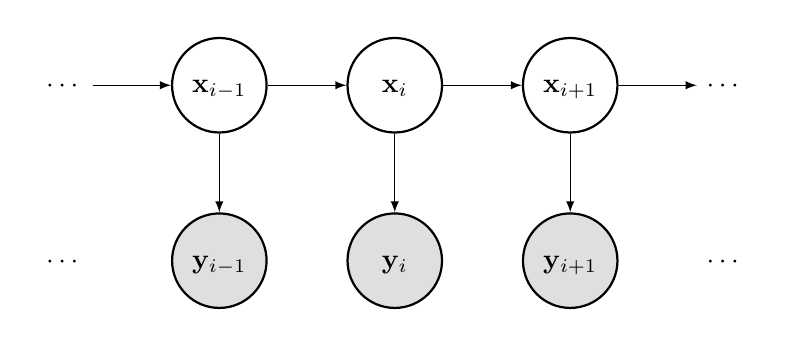
\begin{tikzpicture}[>=latex,text height=1.5ex,text
    depth=0.25ex,ampersand replacement=\&] 
    \matrix[row sep=1cm,column sep=1cm] {
      % first line: hidden continuous state
      \node (x_k-2) {$\cdots$}; \&
      \node (x_k-1) [state] {$\mathbf{x}_{i-1}$}; \&
      \node (x_k)   [state] {$\mathbf{x}_i$};     \&
      \node (x_k+1) [state] {$\mathbf{x}_{i+1}$}; \&
      \node (x_k+2) {$\cdots$};
      \\
      % Second line: Measurement
      \node (y_k-2) {$\cdots$}; \&        
      \node (y_k-1) [measurement] {$\mathbf{y}_{i-1}$}; \&
      \node (y_k)   [measurement] {$\mathbf{y}_i$};     \&
      \node (y_k+1) [measurement] {$\mathbf{y}_{i+1}$}; \&
      \node (y_k+2) {$\cdots$};
      \\
    };
    % The diagram elements are now connected through arrows:
    \path[->]
    (x_k-2) edge (x_k-1)
    (x_k-1) edge (x_k)	
    (x_k)   edge (x_k+1)	
    (x_k+1)   edge (x_k+2)	
    (x_k-1) edge (y_k-1)
    (x_k) edge (y_k)
    (x_k+1)   edge (y_k+1);
  \end{tikzpicture}
  \caption{State-space model. Filled objects are observed, circles
    indicate that both hidden and observed states are
    continuous.\label{fig:ssmod}} 
\end{figure}

In the case where $f_\theta$ and $g_\theta$ are linear with $\epsilon_i$ and
$\eta_i$ normally distributed, \eqref{eq:ssmod} specializes to
\begin{equation}
  \begin{aligned}
    x_{i}&= d+T x_i + R\eta_{i}, 
    & \eta_i &\sim N(0,\ Q),     
    &x_1 &\sim N(x_0,\ P_0).\\
    y_i&= c + Z x_i + \epsilon_i,     
    & \epsilon_i &\sim N(0,\ G) \\
  \end{aligned}
  \label{eq:lgmod}
\end{equation}
where the matrices $d,\ T,\ R,\ c,\ Z,$ and $G$ are allowed to depend
on $\theta$ and can potentially vary (deterministically) with $i$. In this case,
the Kalman filter, \autoref{alg:kalman} \citep[see e.g.][]{Kalman1960,Harvey1990},
can be used to derive closed form 
solutions for the conditional
distributions of the states and to calculate the likelihood of $\theta$
given data. 
\begin{algorithm}[t!]
  \begin{singlespace}
  \caption{Kalman filter: estimate $x_i$ conditional on
    $\{y_j\}_{j=1}^i$, for all $i=1,\ldots,n$ and calculate the log likelihood
    for $\theta$\label{alg:kalman}}
  \begin{algorithmic}
    \STATE {\bf Input:} $Y$, $x_0$, $P_0$, $d,\ T,\ R,\ c,\ Z,$ and $G$
    \STATE $\ell(\theta) \leftarrow 0$ \COMMENT{Initialize the log-likelihood}
    \FOR{$i=1$ to  $n$}
    \STATE $H = RQR'$ \COMMENT{Effective state variance}
    \STATE $\begin{aligned}\varx_{i}
      &\leftarrow d + T x_{i-1|i-1}, & P_i &\leftarrow H + T P_{i-1|i-1}
      T'\end{aligned}$ \COMMENT{Predict current state}
    \STATE $\begin{aligned}\widetilde{y}_i
      &\leftarrow c + Z \varx_i, & F_i &\leftarrow G + Z P_i
      Z'\end{aligned}$ \COMMENT{Predict current observation}
    \STATE $\begin{aligned}v_i&\leftarrow y_i-\widetilde{y}_i& K_i&
      \leftarrow P_i Z' F^{-1}\end{aligned}$ \COMMENT{Forecast error and 
    Kalman gain}
    \STATE $\begin{aligned} x_{i|i}
      &\leftarrow \varx_i + K_i v_i, & P_{i|i} &\leftarrow P_i - P_iZ'
      K_i\end{aligned}$ \COMMENT{Update}
    \STATE $\ell(\theta) = \ell(\theta) -v_i'F^{-1}v_i - \log(|F_i|)$
    \ENDFOR
    \RETURN $\widetilde{Y}=\{\widetilde{y}_i\}_{i=1}^n,\ \varx=\{\varx_i\}_{i=1}^n,\
    \widetilde{X}=\{x_{i|i}\}_{i=1}^n,\ P=\{P_i\}_{i=1}^n,\
    \widetilde{P}=\{P_{i|i}\}_{i=1}^n,\ \ell(\theta)$
  \end{algorithmic}
\end{singlespace}
\end{algorithm}

% However, in many applications, researchers are not so
% lucky. For nonlinear  or non-Gaussian models, approximate solutions
% exist using the particle filter and its derivatives (see for
% example~\citet{Kitagawa1987,Kitagawa1996}
% and~\citet{DoucetDe-Freitas2001} for an exposition of the particle
% filter and~\citet{KoyamaPerez-Bolde2010}
% and~\citet{DejongDharmarajan2009a} for improvements).

While \autoref{alg:kalman} returns the likelihood for $\theta$, 
$\varx_i$ and $P_i$ represent the mean and variance of the conditional distribution
of the unobserved component given only the observations
$\{y_j\}_{j=1}^i$: $\varx_i=\Expect{x_i\given y_1\ldots,y_i}$ and
$P_i=\Var{x_i\given y_1,\ldots,y_i}$. To
incorporate all future observations into these estimates, the Kalman
smoother is required.
\begin{algorithm}[t!]
  \begin{singlespace}
  \caption{Kalman smoother (Rauch-Tung-Striebel): estimate $\hat{X}$ conditional on
    $Y$\label{alg:kalman-smoother}} 
  \begin{algorithmic}
    \STATE {\bf Input:} $\varx$, $\widetilde{X}$, $P$, $\widetilde{P}$,
    $T,$ $c$, $Z$.
    \STATE $t=n$,
    \STATE $\hat{x}_{n}\leftarrow \widetilde{x}_n$, 
    \WHILE{$t>1$}
    \STATE $\hat{y}_i \leftarrow c + Z\hat{x}_i,$
    \COMMENT{Predict observation vector}
    \STATE $\begin{aligned} e &\leftarrow \hat{x}_i -
      \varx_i, & V &\leftarrow P_i^{-1}\end{aligned}$,
    \STATE $t\leftarrow i-1$, \COMMENT{Increment}
    \STATE $\hat{x}_i = \widetilde{x}_i + \widetilde{P}_i T Ve $ 
    \ENDWHILE
    \RETURN $\widehat{Y}=\{\hat{y}_i\}_{i=1}^n, \hat{X}=\{\hat{x}_i\}_{i=1}^n$
  \end{algorithmic}
\end{singlespace}
\end{algorithm}
There are many different smoother algorithms tailored for different
applications. \autoref{alg:kalman-smoother}, due
to~\citet{RauchStriebel1965}, is often referred to as the classical
fixed-interval smoother~\citep{AndersonMoore1979}. It produces only
the unconditional expectations of the hidden state
$\hat{x}_i=\Expect{x_i\given y_1,\ldots,y_n}$ for the sake of
computational speed. This version is more appropriate for inference in
the type of switching models we discuss below.


Linear Gaussian state-space models can be made quite flexible
by expanding the state vector or allowing the parameter matrices to
vary with time. Furthermore, this general form encompasses many
standard time series models: ARIMA models, ARCH and GARCH models,
stochastic volatility models, exponential smoothers, and
more~\citep[see][for many other
examples]{DurbinKoopman2001}. Nonlinear, non-Gaussian versions have
been extensively
studied~\citep{DurbinKoopman1997,Fuh2006,Kitagawa1987,Kitagawa1996}
and algorithms for filtering, smoothing, and parameter estimation have
been derived~\citep[e.g.,][]{KoyamaPerez-Bolde2010,AndrieuDoucet2010}. 
However, these models are less useful
for change-point detection or other forms of discontinuous behavior
when the times of discontinuity are unknown. 

To remedy this deficiency, one can use a switching state-space
model as shown in \autoref{fig:switchss}. Here, we assume $S$ is a
hidden, discrete process with Markovian dynamics. Then, the value of
the hidden state at time $t$, $s_i=k$ say, can determine the evolution of
the continuous model at time $t$. The graphical model in
\autoref{fig:switchss} gives the conditional independence properties
we will use in our model for musical interpretation, but this
represents just one of many possibilities. Switching state-space models have a long
history with many applications from
economics~\citep{KimNelson1998,Kim1994,Hamilton2011} to speech
processing~\citep{FoxSudderth2011} to animal
movement~\citep{PattersonThomas2008,BlockJonsen2011}. An excellent
overview of the history, typography, and algorithmic developments can
be found in~\citep{GhahramaniHinton2000}. In \eqref{eq:lgmod}, the
parameter matrices were not time varying. In our switching model, we
allow the switch states $s_i, s_{i-1}$, along with the parameter
vector $\theta$, to determine the specific dynamics at time $t$:
\begin{equation}
  \begin{aligned}
    x_1 &\sim N(x_0,\ P_0),\\
    x_{i+1}&= d(s_i,s_{i-1})+T(s_i,s_{i-1}) x_i +
    R(s_i,s_{i-1})\eta_i, 
    & \eta_i &\sim N(0,Q(s_i,s_{i-1})),\\
    y_i&= c(s_i) + Z(s_i) x_i + \epsilon_i, & \epsilon_i &\sim N(0, G(s_i)).
  \end{aligned}
\end{equation}
In other words, the hidden Markov (switch) state determines which parameter
matrices govern the evolution of the system. 






\begin{figure}
  \centering
  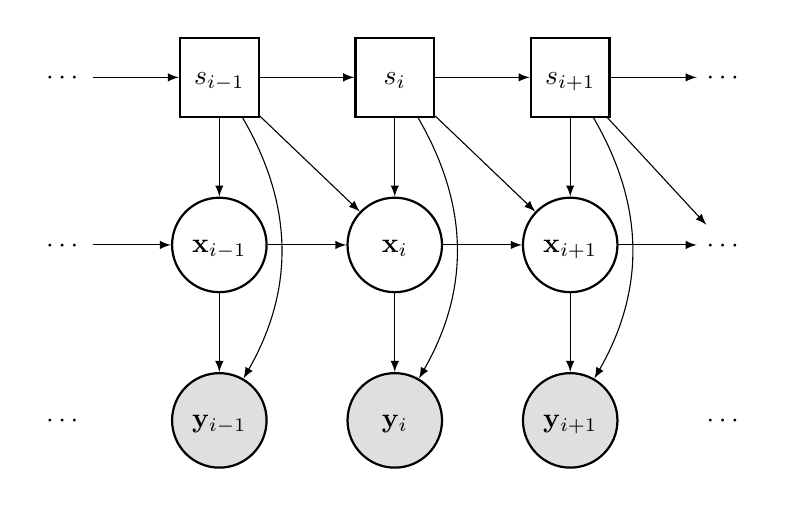
\begin{tikzpicture}[>=latex,text height=1.5ex,text depth=0.25ex,ampersand replacement=\&]
    % The various elements are conveniently placed using a matrix:
    \matrix[row sep=1cm,column sep=1cm] {
      % First line: Switch state
      \node (s_k-2)  {$\cdots$}; \&
      \node (s_k-1) [switch]{$s_{i-1}$}; \&
      \node (s_k)   [switch]{$s_i$};     \&
      \node (s_k+1) [switch]{$s_{i+1}$}; \&
      \node (s_k+2) {$\cdots$};
      \\
      % Second line: hidden continuous state
      \node (x_k-2) {$\cdots$}; \&
      \node (x_k-1) [state] {$\mathbf{x}_{i-1}$}; \&
      \node (x_k)   [state] {$\mathbf{x}_i$};     \&
      \node (x_k+1) [state] {$\mathbf{x}_{i+1}$}; \&
      \node (x_k+2) {$\cdots$};
      \\
      % Third line: Measurement
      \node (y_k-2) {$\cdots$}; \&        
      \node (y_k-1) [measurement] {$\mathbf{y}_{i-1}$}; \&
      \node (y_k)   [measurement] {$\mathbf{y}_i$};     \&
      \node (y_k+1) [measurement] {$\mathbf{y}_{i+1}$}; \&
      \node (y_k+2) {$\cdots$};
      \\
    };
    % The diagram elements are now connected through arrows:
    \path[->]
    (s_k-2) edge (s_k-1)
    (s_k-1) edge (s_k)	
    (s_k)   edge (s_k+1)	
    (s_k+1)   edge (s_k+2)	
    
    (x_k-2) edge (x_k-1)
    (x_k-1) edge (x_k)	
    (x_k)   edge (x_k+1)	
    (x_k+1)   edge (x_k+2)	
    
    (s_k-1) edge (x_k-1)
    (s_k) edge (x_k)
    (s_k+1)   edge (x_k+1)
    
    (x_k-1) edge (y_k-1)
    (x_k) edge (y_k)
    (x_k+1)   edge (y_k+1)
    
    (s_k-1) edge (x_k)
    (s_k) edge (x_k+1)
    (s_k+1)   edge (x_k+2)
    
    (s_k-1) edge[bend left] (y_k-1)
    (s_k) edge[bend left] (y_k)
    (s_k+1)   edge[bend left] (y_k+1)
    ;
  \end{tikzpicture}
  \caption{Switching state space model. Filled objects are observed,
    rectangles are discrete, and circles are continuous.\label{fig:switchss}}
\end{figure}






\subsection{A model for tempo decisions}


In musical scores, tempi (the Italian plural of {\em tempo}) may be
marked at various points throughout a piece of music. The
beginning can be either explicit, with a metronome marking to
indicate the number of beats per minute (bpm), and/or with some words
(e.g. Adagio, Presto, Langsam, Sprightly) which indicate an
approximate speed. 
\begin{figure}[t!]
  \centering
  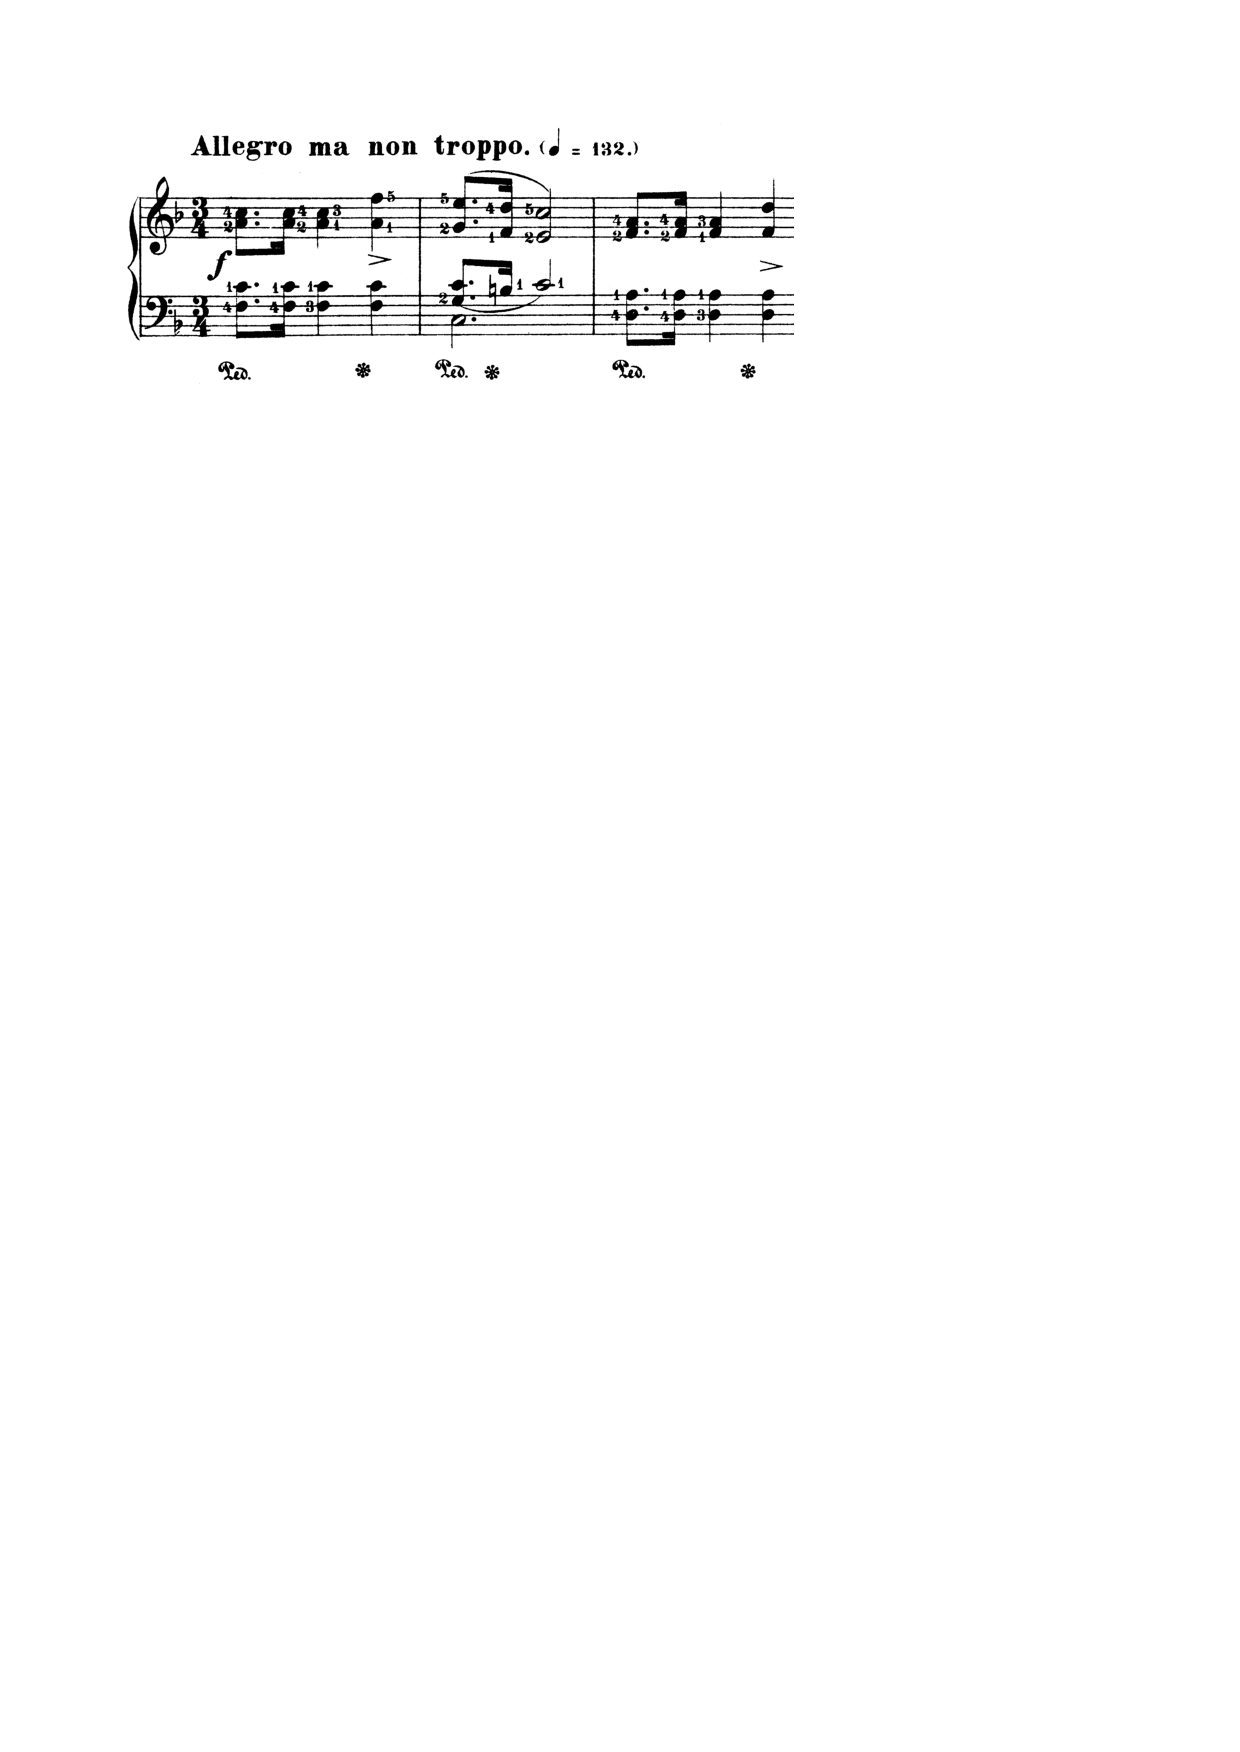
\includegraphics[height=3cm]{mazurka-top.pdf}
  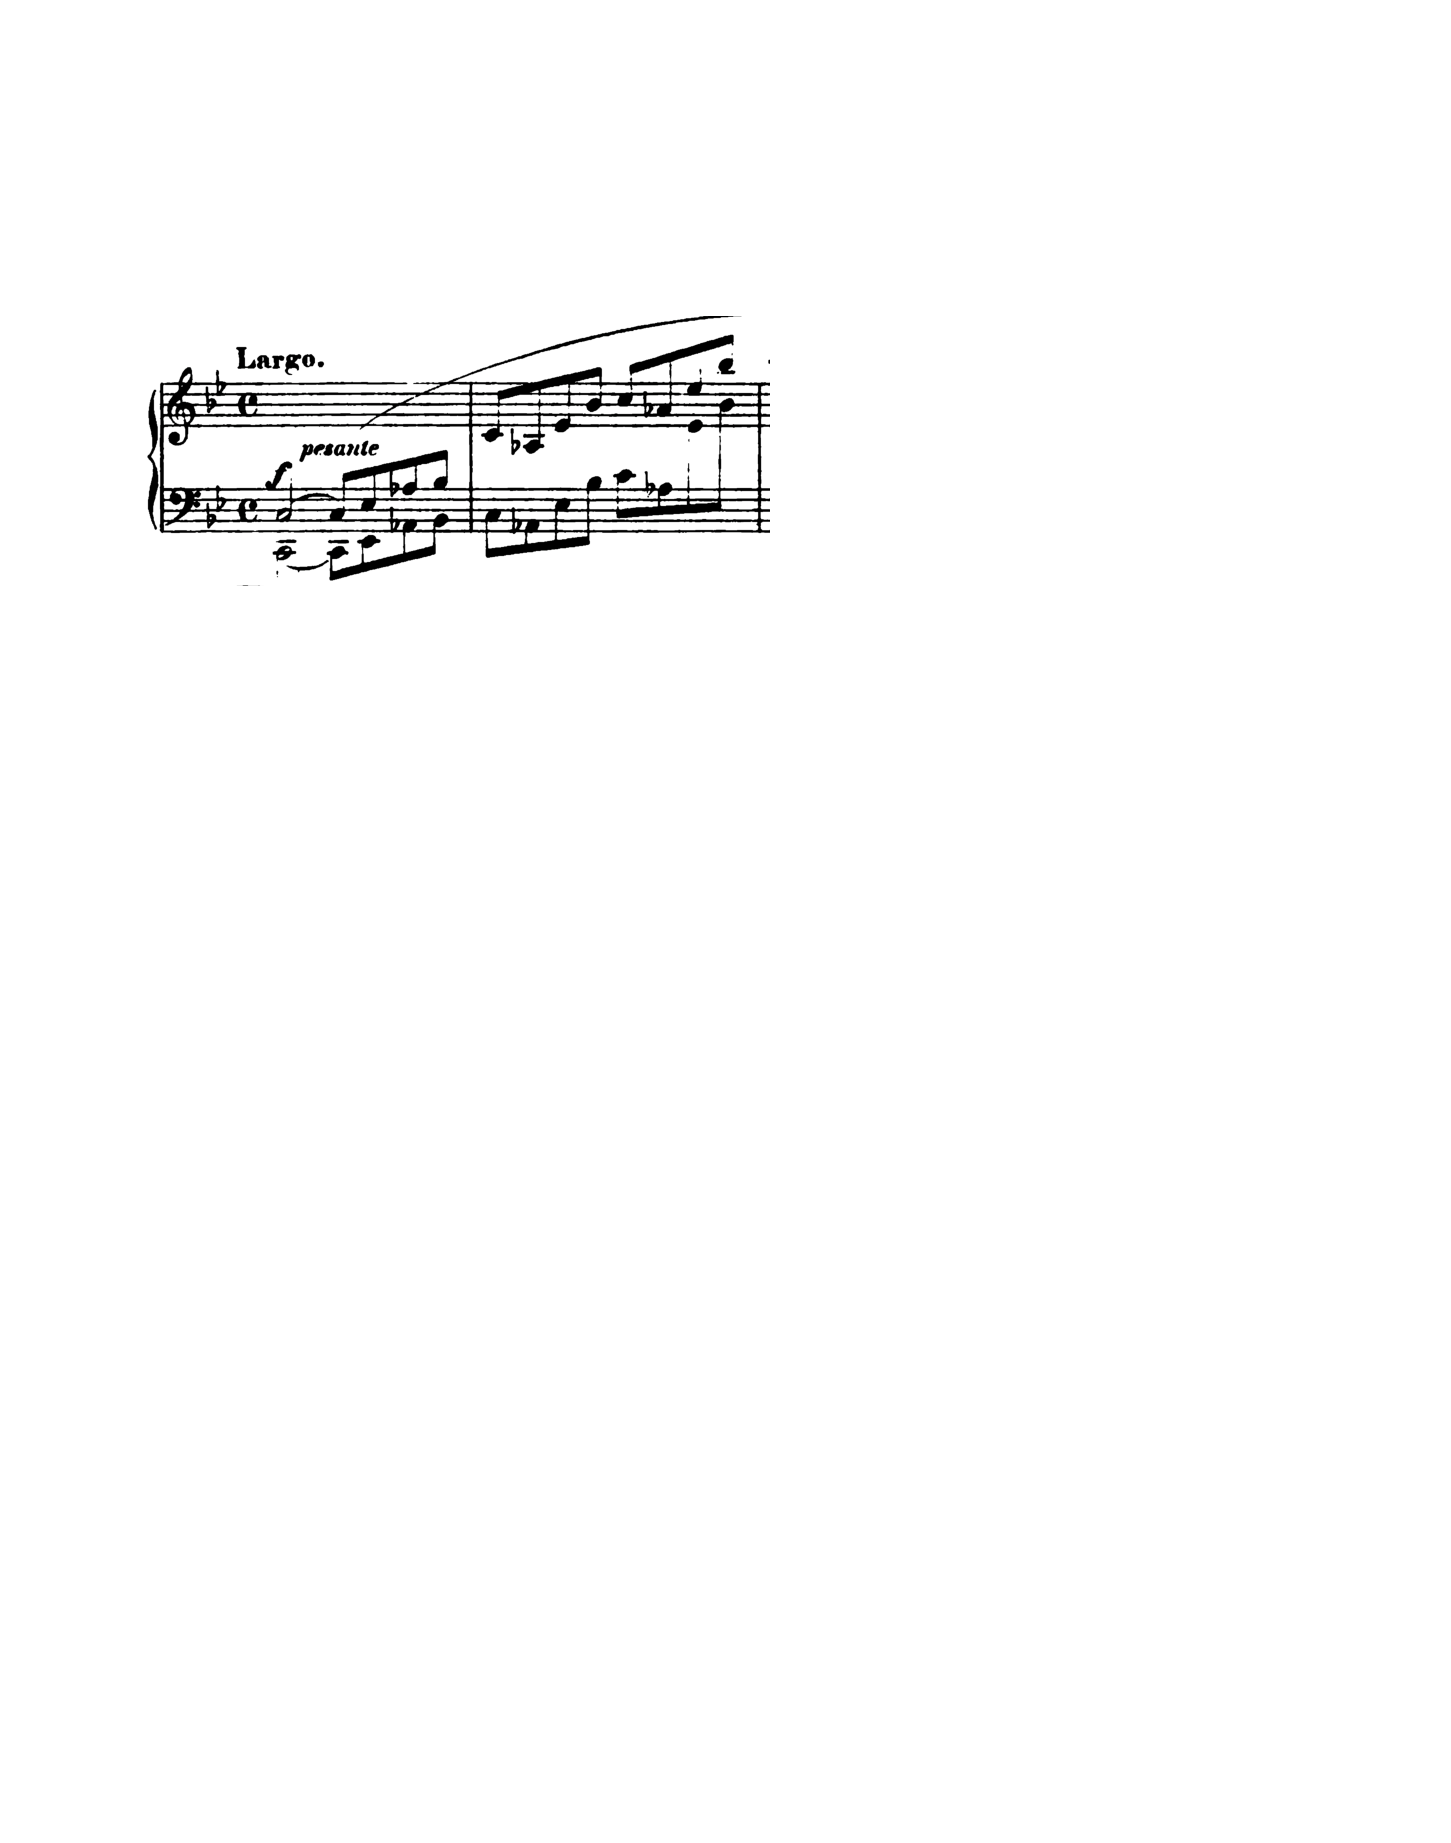
\includegraphics[height=3cm]{ballade-top.pdf}
  \caption{The beginning of two Chopin piano compositions: the Mazurka
    we analyze is on the left while the Ballade No.\ 1, Op.\ 23 is on
    the right.}
  \label{fig:tempo-markings}
\end{figure}
\autoref{fig:tempo-markings} shows the beginning of two Chopin piano
compositions: the Mazurka we analyze and the Ballade No.\ 1, Op.\ 23. The initial tempo of the Mazurka is given with a metronome
marking as well as the Italian phrase {\em Allegro ma non troppo}
(``cheerful, but not too much''). The beginning of the Ballade is simply
marked {\em Largo}, which translates literally as ``broad'' or
``wide''. Obviously, the metronome markings are much more exact,
though even these are often viewed as suggestions rather than
commandments. The metronome markings in most of Beethoven's
compositions, for example, are notoriously fast, and some scholars
believe that his metronome (one of the first ever made) was
inaccurate. Often, compositions will have numerous such markings later
in the piece of music, but these are only some of the ways that tempo
is indicated. Composers will also indicate periods of speeding-up
(\emph{accelerando}) or
slowing-down (\emph{ritardando}).

Absent instructions from the composer, performers generally maintain
(or try to maintain) a steady tempo, and this assumption plays a major
role in our model of tempo decisions. Of course, a normal human being
never plays precisely like a 
metronome, although they may try quite hard to do so. The actual
tempo is therefore best viewed as stochastic, the sum of an
intentional, constant component, plus noise representing inaccuracy
or, perhaps more charitably, unintentional variation which the
listener fails to perceive as ``wrong''. For instance, the example in
\autoref{fig:short-perf} shows the beginning of the piece as performed
by Arthur Rubinstein in a 1961 recording. 
\begin{figure}[t!]
  \centering
  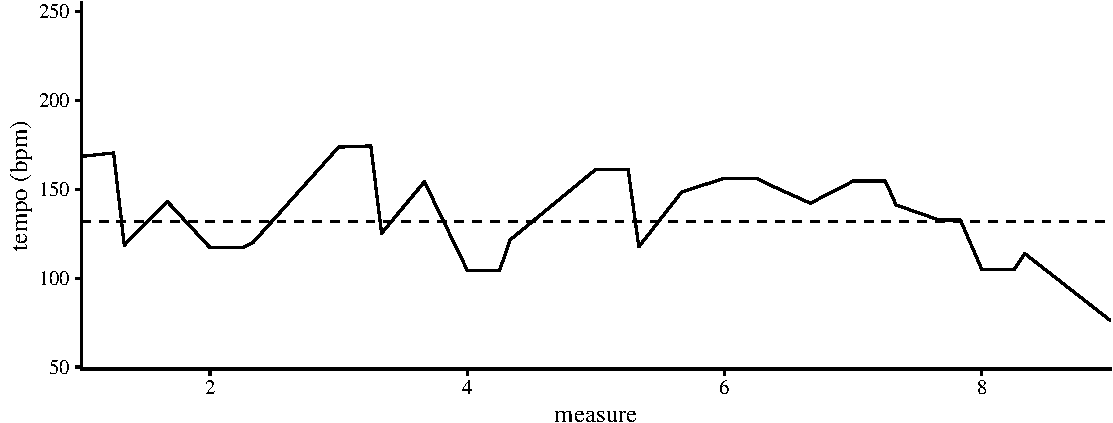
\includegraphics[width=.9\linewidth]{small-rubinstein-1961-1}
  \caption{The solid line shows the observed note-by-note tempo for
    the beginning of the Mazurka as performed by Arthur Rubinstein in
    1961. The dashed line indicates 132 bpm.}
  \label{fig:short-perf}
\end{figure}
The solid line shows the
actual, performed tempo, while the dashed horizontal line is placed at
the indicated tempo of 132 bpm. The figure has three important
lessons: (1) actual tempo varies around intended tempo; (2) 132 bpm is
not necessarily the tempo a performer will choose despite the
indication; and (3) performers have other tempo intentions which are
not marked, like the pronounced slow-down in measures 7--8.

Estimating intended {\em tempi} would be reasonably simple, perhaps, 
if the locations of the tempo changes were known. In such a case,
the average of tempi between changes may be a good estimate as
could the slope of known speed-ups or slow-downs. However, performers
take liberties with these decisions, exactly the liberties we would
like to discover. This suggests employing a switching model with a
small number of discrete states.

We use a model for $S$ on four states
with transition probability
diagram given by \autoref{fig:transmat}.
\begin{figure}[tb!]
  \centering
  \tikzstyle{switch}=[rectangle,
  thick, minimum size=1cm, draw=black]
  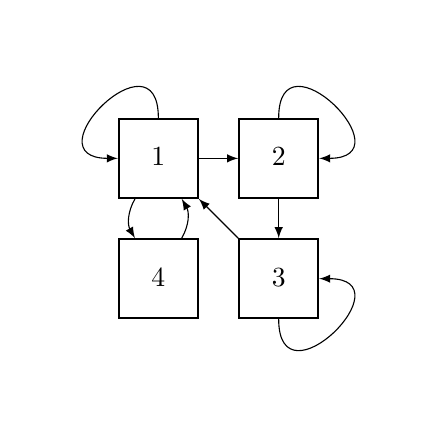
\begin{tikzpicture}[>=latex,text height=1.5ex,text depth=0.25ex]
     \matrix[row sep=0.5cm,column sep=0.5cm] {
       \node (S1) [switch] {$1$}; & \node (S2) [switch] {$2$}; \\
       \node (S4) [switch] {$4$}; & \node (S3) [switch] {$3$}; \\
     };
     \path[->]
     (S1) edge [bend right] (S4)
     (S1) edge (S2)
     (S2) edge (S3)
     (S3) edge (S1)
     (S4) edge [bend right] (S1);
     \draw[->] (S1) to [out=90, in=180,looseness=4] (S1);
     \draw[->] (S2) to [out=90, in=0,looseness=4] (S2);
     \draw[->] (S3) to [out=270, in=0,looseness=4] (S3);
  \end{tikzpicture}
  \caption{Transition diagram. \label{fig:transmat}}
\end{figure}
The 4 switch states correspond to 4 different behaviors for the
performer: (1) constant tempo, (2) speeding up, (3) slowing down, and
(4) single note stress. As shown in the diagram, we only allow certain
transitions for musical reasons and for estimability. The fourth
state, stress, corresponds to {\em tenuto}, a common feature of
musical performance. Such stresses may be marked with a line over the
note in question, but are more often a feature of the performer taste,
corresponding to a longer-than-written duration of a particular
note. Such emphases occur for a variety of musical purposes---emphasis
of the beat in running notes\footnote{\attn{should the amount mean of stress be
  proportional to prevailing tempo, notated duration?}}, the top of a
phrase, a ``landing point'' where a phrase ends, etc.---but are always
within the frame of constant tempo. Thus we allow stress to occur only
after and before notes in state 1. Furthermore, we cannot allow
state 2 to return immediately to state 1, or else ``stress'' could
happen through this pathway. Thus, the entire transition diagram is
fully determined. We discuss some potential improvements at the end
of~\autoref{sec:analys-chop-mazurka}. 


Our data gives $y_i$ as the observed tempo (in bpm) of the note (or
chord) of the $i^{th}$ note onset in Chopin's Mazurka Op.\ No.\ 3. The
hidden continuous variable ($X_i$) is 
taken to be a two component vector with the first component being the
prevailing tempo and the second the amount of acceleration. The amount, or
existence, of acceleration is determined by the current and previous
switch states. We use $l_i$ to denote the musical duration of
a particular note as given by the written score, so, throughout this piece, a quarter-note (\quarternote) has $l_i=1/3$, an
eighth note (\eighthnote) has $l_i=1/6$, etc. This is because each
measure contains three quarter notes. In more complicated
music with changing time signatures or instances where the notation
doesn't necessarily correspond with the time signature, more care
would be required. The observed tempo is already normalized to account
for variable note durations. When the performer is in state 1 (or
transits in and out of state 4), we take the prevailing tempo as
constant with no acceleration: $X_{i+1} = X_i$. 


Corresponding to these configurations, the parameter
matrices are given in \autoref{tab:parmats}
\begin{table}[h!]
\centering
\begin{tabular}[h!]{cc|ccc}
  \hline\hline
  \multicolumn{5}{c}{Transition equation}\\
  \hline
  \multicolumn{2}{c|}{Switch states} & \multicolumn{3}{c}{Parameter
                                      matrices}\\
  $s_i$ & $s_{i-1}$ & $d$ & $T$ & $R$ \\
  \hline
  $S_1$ &  $S_1$ & 0 & $\begin{pmatrix}1&0\\0&0\end{pmatrix}$ 
                 & $\begin{pmatrix}1&0\\0&0\end{pmatrix}$\\
  $S_2$ & $S_1$ & $\begin{pmatrix} l_i\tau_i\\ \tau_i\end{pmatrix}$ 
                                    & $\begin{pmatrix} 1 & 0 \\ 0 &
                                      0 \end{pmatrix}$ 
          & $\begin{pmatrix} 1 & l_i\\ 0 & 1 \end{pmatrix}$\\
  $S_4$ & $S_1$ & $\begin{pmatrix}0\\\varphi_i\end{pmatrix}$ 
                                     & $\begin{pmatrix}1&0\\0&0\end{pmatrix}$
          & $\begin{pmatrix}1&0\\0&1\end{pmatrix}$\\
  $S_2$ & $S_2$ & 0 & $\begin{pmatrix} 1 & l_i \\ 0 & 1 \end{pmatrix}$ 
        & $\begin{pmatrix}1&0\\0&0\end{pmatrix}$\\
  $S_3$ & $S_2$ & $\begin{pmatrix} -l_i\tau_i\\ -\tau_i\end{pmatrix}$ 
                                    & $\begin{pmatrix} 1 & 0 \\ 0 &
                                      0 \end{pmatrix}$ 
          & $\begin{pmatrix} 1 & l_i\\ 0 & 1 \end{pmatrix}$\\
  $S_1$ & $S_3$ & $\begin{pmatrix} \mu_i\\0\end{pmatrix}$ & 0
          & $\begin{pmatrix} 1 & 0\\ 0 & 0 \end{pmatrix}$\\
  $S_3$ & $S_3$ & 0& $\begin{pmatrix} 1 & l_i \\ 0 & 1 \end{pmatrix}$ 
        & $\begin{pmatrix}1&0\\0&0\end{pmatrix}$\\
  $S_1$ &  $S_4$ & 0 & $\begin{pmatrix}1&0\\0&0\end{pmatrix}$ 
        & $\begin{pmatrix}1&0\\0&0\end{pmatrix}$\\
  \hline\hline
  \multicolumn{5}{c}{Measurement equation}\\
  \hline
  \multicolumn{2}{c|}{Switch states} & \multicolumn{3}{c}{Parameter
                                      matrices}\\
  $s_i$ && $c$ & $Z$ & $G$\\
  \hline
  $S_4$ & & 0 & $\begin{pmatrix} 1 & 1 \end{pmatrix}$ &
                                                                  $\sigma^2_\epsilon$\\
  else && 0 & $\begin{pmatrix} 1 & 0 \end{pmatrix}$ &
                                                                  $\sigma^2_\epsilon$\\
  \hline\hline
\end{tabular}
\caption{Parameter matrices of the switching state space model.\label{tab:parmats}}
\end{table}
Finally, 
\[
Q=\begin{cases}\begin{pmatrix} \sigma^2_1 &
    0\\0&\sigma^2_4\end{pmatrix} & (s_i,\ s_{i-1})=(S_4,\ S_1)\\
                \begin{pmatrix} \sigma^2_3 &
                        0\\0&\sigma^2_4\end{pmatrix} & (s_i,\ s_{i-1})=(S_1,\ S_3)\\
\begin{pmatrix} \sigma^2_1 &
    0\\0&\sigma^2_2\end{pmatrix} & \textrm{else}.
\end{cases}
\] 
So for any performance, we want to be able to estimate
the following parameters: $\sigma_1^2$, $\sigma_2^2$, $\sigma^2_4$,
$\sigma_\epsilon^2$, the probabilities of the transition matrix (there
are 4), and vectors $\mu$, $\tau$, and $\varphi$. These last three
will be of different lengths depending on the number of times the
state is visited. Lastly, we have the initial state distributions
\[
x_1\sim\begin{cases} N\left( \begin{pmatrix}\mu_1\\0\end{pmatrix}
  ,\ \begin{pmatrix} \sigma^2_1 & 0\\0 & 0
  \end{pmatrix}\right) & s_1=S_1\\
N\left( \begin{pmatrix}\mu_1\\\tau_1\end{pmatrix}
  ,\ \begin{pmatrix} \sigma^2_1 & 0\\0 & \sigma^2_2
  \end{pmatrix}\right) & s_1=S_3.\end{cases}
\]
Importantly, this is just one way to write this
model.

\subsection{Penalized likelihood maximization}
\label{sec:penal-likel-maxim}

\subsection{Computational issues}
\label{sec:computational-issues}

The problem with estimating a model like this is that, because the
switch states and the continuous states are both hidden, this becomes
an NP-hard problem. In particular, there are $4^N$ possible paths
through the switch variables, so evaluating the likelihood at all of
them is intractable. Thus, I implemented a particular
approximation. The Beam Search (\autoref{alg:beamsearch}), finds
(greedily) evaluates the most likely path through the switch
states. Another name for the algorithm is Discrete Particle Filter
(\texttt{dpf}). Once we have those, \texttt{getLogLike} returns the
negative 
loglikelihood of the data associated with that path. So for any
configuration of parameters, we would form the matrices
(\texttt{yupengMats}) then find the best path (\texttt{dpf}) then
evaluate the likelihood of that path (\texttt{getLogLike}). We can
then optimize over parameters using any variety of numerical
optimization technique. However, when I have tried this, I always get
infinite likelihood.

For this model, the dpf is more easily specified if we make the
measurement equation depend only on the current state and not the
previous state. For this reason, the code uses 16 states rather than
4. One can always change a Markov model in this way.

\begin{algorithm}[t!]
  \caption{Beam search\label{alg:beamsearch}}
  \begin{algorithmic}[1]
  \STATE {\bfseries Input:}
  Initial parameters of the matrices. Integer beam width $B$.
  \FOR{$i=1$ {\bfseries to} $N$} 
  \STATE (\texttt{dpf} performs 1-step of the following);
  \STATE For each current path, calculate the 1-step likelihood for
  moving to each potential switch (\texttt{kf1step})\;
  \STATE Multiply the likelihood by the probability of transitioning
  to that switch state\;
  \STATE Multiply by the previous path weights $w$\;
  \STATE If $\norm{w}_0>B$, resample the weights\;
  (\texttt{resampleSubOptimal}) to get $B$ non-zero weights which
  add to 1.\;
  \STATE Keep only those paths corresponding to the non-zero weights\;
  \ENDFOR
  \STATE Return $B$ paths through the switch space along with their weights.\;
\end{algorithmic}
\end{algorithm}


\section{Analysis of Chopin's Mazurka Op.\ 68 No.\ 3}
\label{sec:analys-chop-mazurka}

\section{Discussion}
\label{sec:discussion}




\bigskip
\begin{center}
{\large\bf SUPPLEMENTARY MATERIAL}
\end{center}

\begin{description}

\item[R-package ``dpf'':] R-package containing code to perform the
  methods described in the article. The package also contains all data
  sets used as examples in the article. (GNU zipped tar)

\end{description}




\bibliographystyle{agsm}
\bibliography{AllReferences}
\end{document}
